\documentclass{article}
\usepackage{graphicx} % Required for inserting images
\graphicspath{ {./Images/} }
\usepackage{amssymb}
\usepackage{pdfpages}
\newcommand{\insertslide}[3]{
\begin{center}
    \fbox{\includegraphics[page=#2,scale=#3]{#1}}
\end{center}
}
% \insertslide{Slides/CM1.pdf}{1} to insert first page of CM1.pdf, for example.
\usepackage{amsmath}
\renewcommand{\familydefault}{\sfdefault}

\title{Synthèse LMAPR1491}
\author{Quentin Bodart}
\date{Q1 2024-2025}

\begin{document}
\maketitle
\tableofcontents
\pagebreak

\section*{Introduction}
    Le but de la physique statistique est d'exprimer les propriétés d'un matériau (grandeurs thermodynamiques) à partir d'une moyenne prise sur la dynamique des constituants (atomes/molécules) du système.
    Elle permet, par le bias d'un \textbf{Postulat Statistique}, de déterminer le comportement d'un matériau via la construction d'une \textbf{Physique statistique} de manière simplifiée.

\section{CM1 : Théorie Cinétique des Gaz (TCG)}
    La \textbf{Théorie Cinétique des Gaz} applique les lois de la mécanique classique (Newton) aux composants microscopiques du gaz de manière "statistique". Elle ne peut s'appliquer qu'à un gaz constitué d'un grand nombre de molécules identiques, se meuvant aléatoirement, et dont la distance moyenne est bien plus grande que leurs dimensions. Elle considère les collisions entre molécules et les parois comme élastiques.

    \subsection{Pression sur un réservoir}
        La force exercée par une molécule sur la paroi est égale au taux de transfert de quantité de mouvement à la paroi.
        Considérant la distance entre deux parois $d$ et une quantité de mouvement $p = 2 mv_{x i}$ où $v_{x i}$ désigne la vitesse de la particule i dans la direction de l'axe x, on peut écrire:
        $$
        F_i = \frac{2mv_{x i}}{2 d/v_{x i}} = \frac{mv_{x i}^2}{d}
        $$ \\
        où $2 d/v_{x i}$ désigne le temps que prend une particule à faire un aller-retour dans le contenant. \\\\
        La force totale exercée par toutes les $N$ molécules sur la paroi est donc:
        $$
        F = \sum F_i = \frac{m}{d} (v_{x1}^2 + v_{x2}^2 + ... + v_{xN}^2)
        $$
        La valeur moyenne du carré de la vitesse dans la direction x pour N molécules vaut :
        $$
        \overline{v_x^2} = (v_{x1}^2 + v_{x2}^2 + ... + v_{xN}^2) / N
        $$
        La force totale sur la paroi peut donc s'écrire :
        $$
        F = \frac{Nm}{d} \overline{v_x^2}
        $$
        Et comme le mouvement est complètement aléatoire :
        $$
        \overline{v^2} = \overline{v_x^2} + \overline{v_y^2} + \overline{v_z^2} = 3\overline{v_x^2}
        $$
        La force totale peut donc s'écrire:
        $$
        F = \frac{N}{3} (\frac{m\overline{v^2}}{d})
        $$ 
        On peut enfin calculer la pression totale exercée par le gaz sur le réservoir :
        $$
        P = \frac{F}{A} = \frac{F}{d^2} = \frac{2}{3} (\frac{N}{V}) (\frac{1}{2}m\overline{v^2})
        $$
        A partir de ce résultat et de la loi des gaz parfaits, on peut trouver que la température est directement liée à l'énergie cinétique moyenne des molécules :
        $$
        \frac{1}{2}m\overline{v^2} = \frac{3}{2} k_B T
        $$
    
    \subsection{Chaleur spécifique molaire de gaz idéaux}
        Un gaz ne possède pas une chaleur spécifique unique. Cepandant, on peut trouver les chaleurs spécifiques pour une transformation \textbf{isochore} ou \textbf{isobare}.
        \begin{itemize}
            \item $c_V$ = chaleur spécifique molaire à \textbf{volume constant}
            \item $c_P$ = chaleur spécifique molaire à \textbf{pression constante}
        \end{itemize}
        Les chaleurs nécessaires pour augmenter la température du gaz de $\Delta T$ parc ces deux processus sont respectivement:
        \begin{itemize}
            \item $Q_V = n c_V \Delta T$
            \item $Q_P = n c_P \Delta T$
        \end{itemize}

        \subsubsection{Valeur de $c_V$}
            La chaleur transférée à un système à volume constant :
            $$
            Q = n c_V \Delta T = \Delta E_{int}
            $$
            car à volume constant, le travail est nul. \\\\
            En supposant que l’énergie interne soit égale à l’énergie de translation totale des molécules, alors
            $$
            \Delta E_{int} = \frac{3}{2} n R \Delta T 
            $$
            donc,
            $$
            c_V = \frac{\Delta E_{int}}{n \Delta T} = \frac{3}{2} R
            $$
        
        \subsubsection{Valeur de $c_P$}
            La chaleur transférée à un système à pression constant :
            $$
            Q = n c_P \Delta T = \Delta E_{int} - W
            $$\\\\
            En supposant que l’énergie interne soit égale à l’énergie de translation totale des molécules, alors
            $$
            \Delta E_{int} = \frac{3}{2} n R \Delta T,
            $$
            $$
            W = -P \Delta V = -n R \Delta T
            $$
            donc,
            $$
            c_P = \frac{\Delta E_{int} - W}{n \Delta T} = \frac{5}{2} R
            $$
    \subsection{Comparaison avec des gaz réels}
        En se basant sur les valeurs de $c_P$ et $c_V$ précédemment trouvées, on a 
        $$
        c_P - c_V = R
        $$
        et
        $$
        \gamma = c_P / c_V = 1.667
        $$
        On peut observer dans la table ci-dessous que ces valeurs correspondent bien aux gaz mono-atomiques.\\
        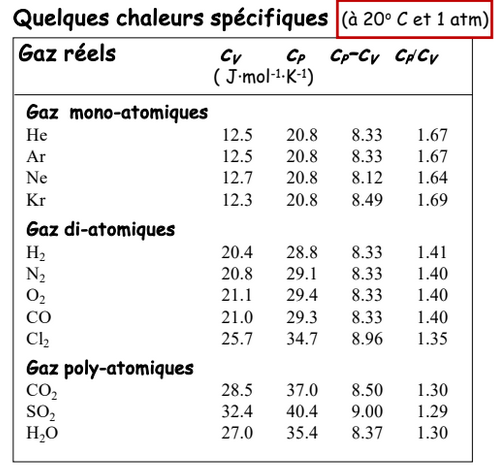
\includegraphics[scale = 0.5]{chaleurs_specifiques.png}\\
        Cependant, pour les gaz di- ou poly-atomiques, le désaccord est principalement dû à l'hypothèse erronée qui mentionne que \textit{l’énergie interne d’un gaz est égale à l’énergie cinétique de translation totale des molécules.}\\
        Cette hypothèse est \textbf{uniquement valable dans le cas monoatomique} ! 
        Dans le cas di- ou poly-atomique, la molécule peut tourner et vibrer autour de son centre de masse, engendrant de l’énergie de rotation et de vibration. 
        \textbf{Ces énergies additionnelles doivent être inclues dans l’énergie interne du système.}\\\\
        Considérons un gaz di-atomique dont les molécules ont la forme d'une haltère :\\
        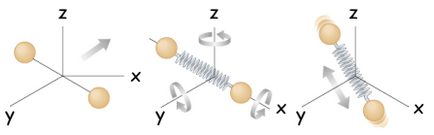
\includegraphics{gaz_diatomique.png}\\
        Considérant que l'énergie interne est partagée équitablement entre chaque degré de liberté (c.f. Théorème d'équipartition de l'énergie), on aurait $c_V = (8/2)R = 33.216 \: J.mol^{-1}.K^{-1}$, qui est bien supérieur à ce qui est observé dans la table précédente !
        Si l'on contourne le théorème d'équipartion, et que l'on considère que la \textbf{rotation selon l'axe x et les vibration selon les axes y et z sont négligeables}, on obtient \textbf{approximativement la bonne réponse.}
        Le théorème d'équipartition ne tient pas non plus compte de la \textbf{variation en température de la chaleur spécifique molaire}. \\\\
        L’insuccès du théorème d’équipartition lors de la prédiction des chaleurs spécifiques molaires de gaz di- et poly-atomiques réside dans l’inadéquation de la mécanique classique et du théorème d'équipartition pour l’étude de systèmes moléculaires. 
        Un modèle plus adéquat serait basé sur la mécanique quantique.
    
    \subsection{Distibution de Maxwell-Boltzmann}
        Les chocs inter-moléculaires redistribuent en permanence la direction et la vitesse de celles-ci. Les vitesses sont donc \textbf{distribuées statistiquement}.\\\\
        Appellons $\phi_x (v_x)$, la fraction des molécules dont la composante x de la vitesse est inférieure ou égale à $v_x$ (mêmes définitions pour y et z).
        Les composantes de vitesse peuvent varier de $-\infty$ à $+\infty$. \\
        Appellons $\phi(v)$, la fraction des molécules dont la vitesse totale est inférieure ou égale à $v$.
        La vitesse $v$ peut varier de 0 à $+\infty$. \\
        $\phi$, $\phi_x$, $\phi_y$ et $\phi_z$ sont toutes des \textbf{Cumulative Distribution Function} (c.f. LEPL1109).
        Les dérivées de ce fonctions nous donne les \textbf{Probability Density Function} (ou distribution de vitesse) $f$, $f_x$, $f_y$ et $f_z$.
        $$
        f_x(v_x) = \frac{\partial \Phi_x}{\partial v_x} \; \; f_y(v_y) = \frac{\partial \Phi_y}{\partial v_y} \; \; f_y(v_y) = \frac{\partial \Phi_y}{\partial v_y}
        $$
        $$
        f(v) = \frac{\partial \Phi}{\partial v}
        $$
        Pour un système \textbf{isotrope}:
        $$
        f_x(v_x) = f_y(v_y) = f_z(v_z) = f_{xyz}
        $$
        Basée sur ces valeurs, via un raisonnement qu'il n'est pas nécessaire de retenir, on obtient la distribution de Maxwell-Boltzmann :
        $$
        N_v = N f(v) = 4 \pi N \left( \frac{m}{2\pi k_B T} \right) ^{3/2} v^2 e^{-\frac{m v^2}{2 k_B T}}
        $$

\section{CM2 : Eléments de physique statistique}
        \subsection{Espace de phase et points représentatifs}
            Un \textbf{espace de phase} permet de représenter un système par un seul point de cet espace. \\
            %TODO équations de hamilton
            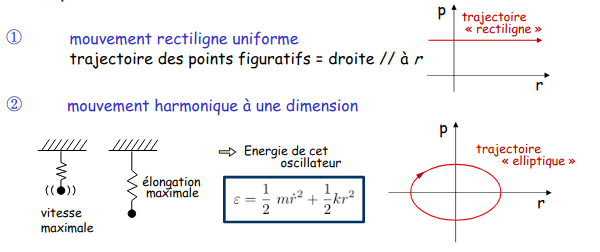
\includegraphics[scale=.5]{espace_de_phase_exs.png} \\
            Dans le cas de la physique statistique, nous travaillons avec un très grand nombe de particules.
            Soit un système conservatif à N particules, le nombre de degrés de liberté de ce système vaut 3N (s’il n’y a pas de liaisons). \\
            On travaillera alors avec un système à 3N degrés de liberté.
            Cependant, cela requiert la connaissance complète du système, ce qui est techniquement impossible.
            De plus, en réalité, aucune mesure d'énergie ne peut fournir une mesure exacte de celle-ci.
            %TODO Probabilité temporelle de l'état d'un système (moyenne temporelle d'une grandeur physique)
        
        \subsection{Notion d'ensemble}
            Sert à passer d'un état temporel à un ensemble d'états à un temps $t_0$
            %TODO Compléter

        \subsection{Postulat d'équiprobabilité}
            Lorsque qu’un système isolé est à l’équilibre, chaque état microscopique
            de ce système, compatible avec son état macroscopique, est également probable.
        
        \subsection{Rappel sur l'entropie}
            Dans un ensemble microcanonique, %TODO
            \begin{itemize}
                \item La différence d'entropie entre un état final et initial peut se calculer en joignant ses deux états par une succession de transformations réversibles.
                \item Un système isolé évolue spontanément dans le sens d'une augmentation de son entropie.
            \end{itemize}
            
            En résumé, l'entropie est : 
            \begin{itemize}
                \item une \textbf{fonction variationelle} déterminant les états d’équilibre de
                systèmes fermés à partir d’un principe mathématique d’extremum.
                \item une \textbf{variable extensive} ($S=S_1 +S_2 +S_3 +...$) comme l’énergie U,
                le volume V, le nombre de moles N, le moment magnétique, etc.
            \end{itemize}
        
        \subsection{Etat microscopique d'un système}
            A tout instant, l’ état microscopique d'un système de particules peut
            être caractérisé par l'ensemble des positions, quantités de mouvement
            et énergies des particules à cet instant.
            En mécanique quantique, si une particule est confinée dans un volume fini,
            elle ne peut posséder qu'un nombre discret de niveaux d'énergie : quantification des niveaux d’énergie.\\
            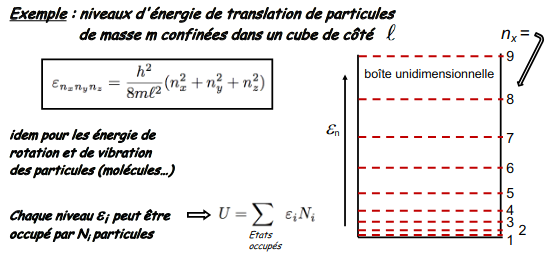
\includegraphics[scale=.8]{niveaux_d_energie.png}

        %TODO Aucun système n'est complètement isolé

        \subsection{Equation de Boltzmann}
            Soit $\Omega$ le nombre d'états microscopiques possibles d'un système vérifiant les contraintes macroscopiques imposées,
            alors il existe une relation vérifiant $S = f(\Omega)$.
            Vu que l'entropie S est \textbf{additive}, et que $\Omega$ est \textbf{multiplicatif}, on a 
            $$
            S = A ln(\Omega)
            $$
            On choisit $A = k_B$, afin d'être en accord avec l'échelle Kelvin de températue.
            L'\textbf{équation de Boltzmann} est donc :
            $$
            S = k_B ln(\Omega)
            $$
        
        \subsection{Modèle d'Einstein du solide cristallin}
            Le modèle d’Einstein consiste en l’hypothèse que chacun des
            Ñ atomes du cristal peut être considéré comme étant attaché à sa position
            d’équilibre par une force harmonique de rappel.
            Chaque atome est libre de vibrer autour de sa
            position d’équilibre dans n’importe laquelle des
            3 directions de l’espace, avec une fréquence
            naturelle $w_0$ . \\\\
            De manière plus réaliste, les atomes du cristal sont attachés 'harmoniquement' (avec des ressorts) aux atomes voisins dans la structure, plutôt
            qu’à des points fixes (position d’équilibre) \\
            Ceci implique que l'on doive distribuer l'énergie interne $U$ en $\frac{U}{\hbar w_0}$ quantas à distribuer entre Ñ atomes.
            On a donc :
            $$
            \Omega = \frac{(3 \tilde N - 1 + \frac{U}{\hbar w_0})!}{(3 \tilde N -1)! \: (\frac{U}{\hbar w_0})!}
            $$
            Et donc :
            $$
            S = k_B ln(\Omega) = k_B [ln(3 \tilde N)! + ln(\frac{U}{\hbar w_0})! - ln(3 \tilde N)! - ln(\frac{U}{\tilde N w_0})]
            $$
            Considérant que $\frac{1}{T} = \frac{\partial S}{\partial U}$, on a l'énergie moyenne par oscillateur :
            $$
            \frac{U}{3 \tilde N} = \frac{\hbar w_0}{e^{\hbar w_0 / k_B T} - 1}
            $$
            On peut enfin calculer $c_V$ dans le modèle d'Einstein : \\
            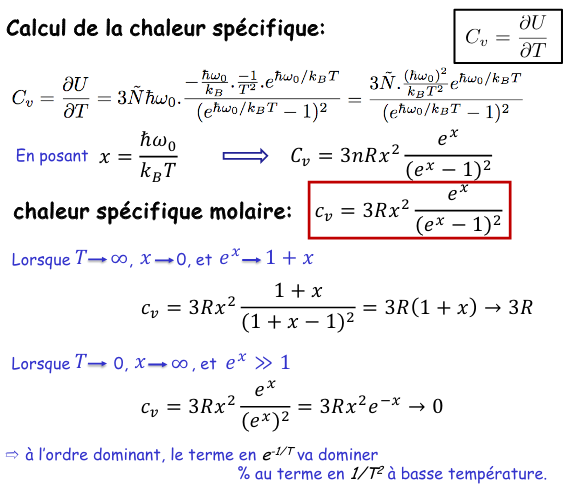
\includegraphics[scale = .5]{c_v_einstein.png}
        %TODO Système à deux états
\pagebreak
\section{CM 3 : Ensemble Canonique et fonction de partition}
    \subsection{Ensemble Canonique}
        \insertslide{Slides/CM3}{2}{.6}
    \subsection{Fonction de partition}
        \insertslide{Slides/CM3}{3}{.6}
        \insertslide{Slides/CM3}{4}{.6}
        \subsubsection{Propriétés de la fonction de partition}
            Une des propriétés les plus importantes de la fonction de partition est qu'elle est \textbf{multiplicative},
            c'est-à-dire que la fonction de partition d'un système (Z barré) est \textbf{équivalente au produit des fonctions de partition
            de chaque constituant} (Z)!\\\\
            Considérons un ensemble composé de $\tilde N$ éléments discernables, alors:
            \begin{itemize}
                \item L’énergie du système est la somme des énergies sur les éléments
                qui sont indépendants, discernables et non-interagissants
                \item Chaque élément peut-être dans un ensemble d’états différents de l'état du système global
                \item Chaque élément ne doit pas être identique que ce soit au niveau
                énergétique ou sur le nombre d’états orbitaux possibles.
            \end{itemize}
            La fonction de partition peut être utilisée avec le formalisme de l'ensemble Canonique
            afin de retrouver bien plus facilement les propriétés de modèles tels que le système à 
            deux états, le modèle d'Einstein ou encore le modèle des gaz parfaits. (c.f. CM3)
    
    \subsection{Densité d'états}
        Dans le formalisme canonique, il est souvent nécessaire d'effectuer la somme
        $$
        \sum_i (...) e^{-\beta E_j}
        $$
        La sommation s’effectue sur tous les états j du système, $E_j$ étant l’énergie du j ème état.\\
        Pour des systèmes macroscopiques, les énergies $E_j$ sont très peu espacées, ce qui permet de remplacer la somme:
        $$
        \sum_i (...) e^{-\beta E_j} \tilde = \int_{E_{min}}^\infty (...) e^{-\beta E} D(E) dE
        $$
        où $E_min$ = Energie de l’état fondamental du système (énergie minimale possible) et
        $D(E)$ = fonction "densité d’état" définie par le nombre d’états dans l’intervalle $dE \rightarrow D(E)dE$

    \subsection{Modèle de Debye}
        Le modèle de Debye reprend le modèle d'Einstein et assigne à chaque oscillateur une fréquence dépendante de la longueur d'onde ($w(\lambda)$).
    
    \subsection{Théorie du corps noir}
        Le problème du corps noir consiste à comprendre et décrire mathématiquement ce qui se passe quand un morceau de fer chauffé passe de la couleur rouge à la couleur blanche, en émettant une quantité de lumière de plus en plus importante.\\\\
        L'intensité lumineuse dégagée par un corps noir est donnée par $I = \sigma T^4$, avec $\sigma$ la constante de Stefan-Boltzmann.\\
        En utilisant le formalisme canonique, on trouve aussi que l'énergie interne d'un corps noir varie en $T^4$.
\pagebreak
\section{CM4 : Potentiel Grand-Canonique}
    \subsection{Formalisme Grand-canonique}
        Le formalisme grand-canonique considère un système relié à un réservoir thermique \textbf{et} à un réservoir de particules.\\
        Après calculs (c.f. Slides/CM4.pdf), on obtient sa fonction de partition :
        $$
        \mathcal{Z} = \sum_{j} e^{-\beta (\epsilon_j - \mu N_j)} = e^{-\beta \Psi}
        $$
        avec\\
        $\Psi = U - TS - \mu \tilde N$ le potentiel grand-canonique,\\
        $\beta = \frac{1}{k_B T}$\\
        $S = - \frac{\partial \Psi}{\partial T}$\\
        (le $\mathcal{Z}$ dans le formalisme grand-canonique est généralement noté avec une double barre)
    
    \subsection{Fluides quantiques}
        Il existe naturellement 2 particules "classiques":
        \begin{itemize}
            \item les \textbf{Fermions} (électrons, protons, neutrons, ...)\\
            Fonction d'onde asymétrique, principe d'exlusion de Pauli,\\ analogie aux \textbf{particules matérielles}
            \item les \textbf{Bosons} (photons, phonons, ...)\\
            Fonction d'onde symétrique, masse nulle, analogie aux \textbf{ondes}
        \end{itemize}

        \subsubsection{Modèle du pré-gaz}
            Gaz de Fermions de spin 1/2 avec 3 états d'énergie ($\epsilon_1$, $\epsilon_2$, $\epsilon_3$) permis, en contact avec un réservoir de Fermions de spin +-1/2.\\
            Les Fermions vont alors respecter la \textbf{distribution de Fermi-Dirac} :
            $$
            f_{n,m_s} = \frac{1}{e^{\beta (\epsilon - \mu)} + 1}
            $$
\pagebreak
        \subsubsection{Fluide idéal de Fermi}
            Extrapolation du modèle du pré-gaz de Fermions :\\ comme le nombre d'états orbitaux d'un fluide de Fermi est très grand, les sommations des fonctions de partition sont remplacées par des intégrations.\\
            On obtient donc :
            $$
            \tilde N = \int_{0}^{\infty} \epsilon^{1/2} f(\epsilon) d\epsilon
            $$
            $$
            U = \int_{0}^{\infty} \epsilon^{3/2} f(\epsilon) d\epsilon
            $$\\\\
            A très haute température, on peut approximer $f(\epsilon) = e^{\beta \mu} e^{- \beta \epsilon}$, et on retrouve donc
            $$
            U = 3/2 k_B T
            $$
            $$
            c_V = 3/2 R
            $$
            ce qui correspond exactement au compertement d'un gaz idéal classique ! \\\\
            A T=0, en définissant une énergie de Fermi (potentiel chimique à température nulle) $\mu_0$, on peut trouver
            $$
            U = 3/5 \tilde N \mu_0
            $$\\\\
            Basé sur les raisonnements précédents, on peut déterminer, après une intégration par partie et un dévellopement de Taylor : 
            $$
            \frac{\tilde N}{\tilde N (T = 0)} = (1 + \frac{\pi^2}{8}(\frac{k_B T}{\mu})^2 + ...)^{2/3}
            $$
            ce qui permet d'écrire :
            $$
            \mu \approx \mu_0 (1 - \frac{\pi^2}{12}(\frac{k_B T}{\mu})^2)
            $$\\
            3 conclusions :
            \begin{itemize}
                \item La température de Fermi ne varie pas
                \item $\mu$ décroit lorsque la température augmente
                \item La chaleur spécifique d'un fluide de Fermi nécéssite un facteur de correction d'environ 10\%
            \end{itemize}
\end{document}